\documentclass{beamer}

% ************************
% * fichier de préambule *
% ************************

% ***** extensions *****
\usepackage[T1]{fontenc}	% Caractères accentués et césure
\usepackage[utf8x]{inputenc}	% Choix de l'encodage
\usepackage{graphicx}		% Paquage pour l'insertion d'images
\usepackage{wrapfig}		% Figures flottantes
\usepackage[french]{babel}	% Support Français
\usepackage{eurosym}		% Signe € qui s'adapte en fonction de la police
\usepackage{fancyhdr}		% En-tête de pages personalisés
\usepackage{color}		% Un peu de couleurs
\usepackage{array}		% Faire des beaux tableaux
% Liens cliquables dans le document
\usepackage[colorlinks=true,linkcolor=black,urlcolor=blue,%
pdftitle={Workshop Space Invaders},pdfauthor={Némunaire}]{hyperref}
\usepackage{amsmath}		% Formules matématiques
\usepackage{listings}           % Mise en forme de code source

% Changement des polices du document
\usepackage{palatino}
\usepackage[sc]{mathpazo}
\linespread{1.05}


% ***** césures particulières *****

\hyphenation{}

% ***** filigrane *****
%\usepackage{eso-pic,rotating}
%\AddToShipoutPicture{%
%\unitlength 1cm
%\put(11,15){%
%\begin{rotate}{45}
%\makebox(0,0){\color{lightgray}\scalebox{3.5}{\Huge BROUILLON}}
%\end{rotate}}
%}

% ***** couleurs perso *****

\definecolor{lightgray}{RGB}{240,240,240}

\definecolor{vert}{RGB}{0,176,80}
\definecolor{verta}{RGB}{79,97,40}
\definecolor{vertb}{RGB}{195,214,155}
\definecolor{vertc}{RGB}{235,241,221}
\definecolor{bleua}{RGB}{31,73,125}
\definecolor{bleub}{RGB}{219,229,241}
\definecolor{rougea}{RGB}{192,80,77}
\definecolor{rougeb}{RGB}{242,220,219}

\definecolor{brown}{RGB}{128,0,0}
\definecolor{blue}{RGB}{0,0,255}
\definecolor{green}{RGB}{0,128,0}
\definecolor{seagreen}{RGB}{69,158,181}


% ***** paramètre de la coloration syntaxique *****
\lstset{language=C++,basicstyle=\ttfamily\footnotesize,%
stringstyle=\ttfamily\color{brown},commentstyle=\color{green},%
%numberstyle=\footnotesize,stepnumber=1,numbersep=7pt,%
backgroundcolor=\color{vertc},frame=single,tabsize=2,breaklines=true,%
breakatwhitespace=false,%
classoffset=0,% Mots clés non reconnus
morekeywords={implicit,override,string,abstract},keywordstyle=\color{blue},%
classoffset=1,% Noms de classes
morekeywords={Value,Convert,Exp,Cst},keywordstyle=\color{seagreen},%
classoffset=0
}

% ***** commandes personnelles *****

\newcommand{\helpbox}[3][bleu]{\vspace{1em}\fcolorbox{#1a}{#1b}{\parbox{.92%
\linewidth}{\hspace{5pt}\textbf{#2~:} #3}}\vspace{0.75em}}
\newcommand{\tp}{workshop}
\newcommand{\Tp}{Workshop}
\newcommand{\svn}{\textsc{svn}}
\makeatletter
\renewcommand{\chapter}{\clearpage%
     \@startsection{chapter}{1}{-0.75em}{\baselineskip}%
     {0.5\baselineskip}{\LARGE\textbf}}
\makeatother
\renewcommand{\thechapter}{\Roman{chapter}}
\renewcommand{\thesection}{\arabic{section}}

% ***** en-têtes et pieds de pages *****
\pagestyle{fancyplain}
	\lhead[\emph{\nouppercase{\leftmark}}]{\emph{\textit{\Tp{} Subversion}}}
	\chead{} 
	\rhead[\emph{\textit{\Tp{} Subversion}}]{\emph{\nouppercase{\leftmark}}}
	\lfoot[]{\small{\textit{GConfs 2010}}}
	\rfoot[\small{\textit{GConfs 2010}}]{}


\begin{document}

\title{Bien commencer son projet}
\author{Aurélien \textit{Aurag} \textsc{Legrand} \and \textsc{GConfs}}
\date{Vendredi 03 décembre 2010}

\begin{frame}
  \begin{center}
    
\includegraphics[scale=0.35]{images/logo}
  \end{center}

  \maketitle
\end{frame}

\begin{frame}
  \tableofcontents
\end{frame}

\section{Introduction}
\begin{frame}{Introduction}
  \begin{center}
    \begin{overlayarea}{\textwidth}{175px}

      \only<1>{
\includegraphics[height=200px]{brainstorming-1.pdf}}
      % Le but de cette conférence, c’est vous aider à bien commencer votre
      % projet. Ben oui, mais c’est quoi ce projet ?
      \only<2>{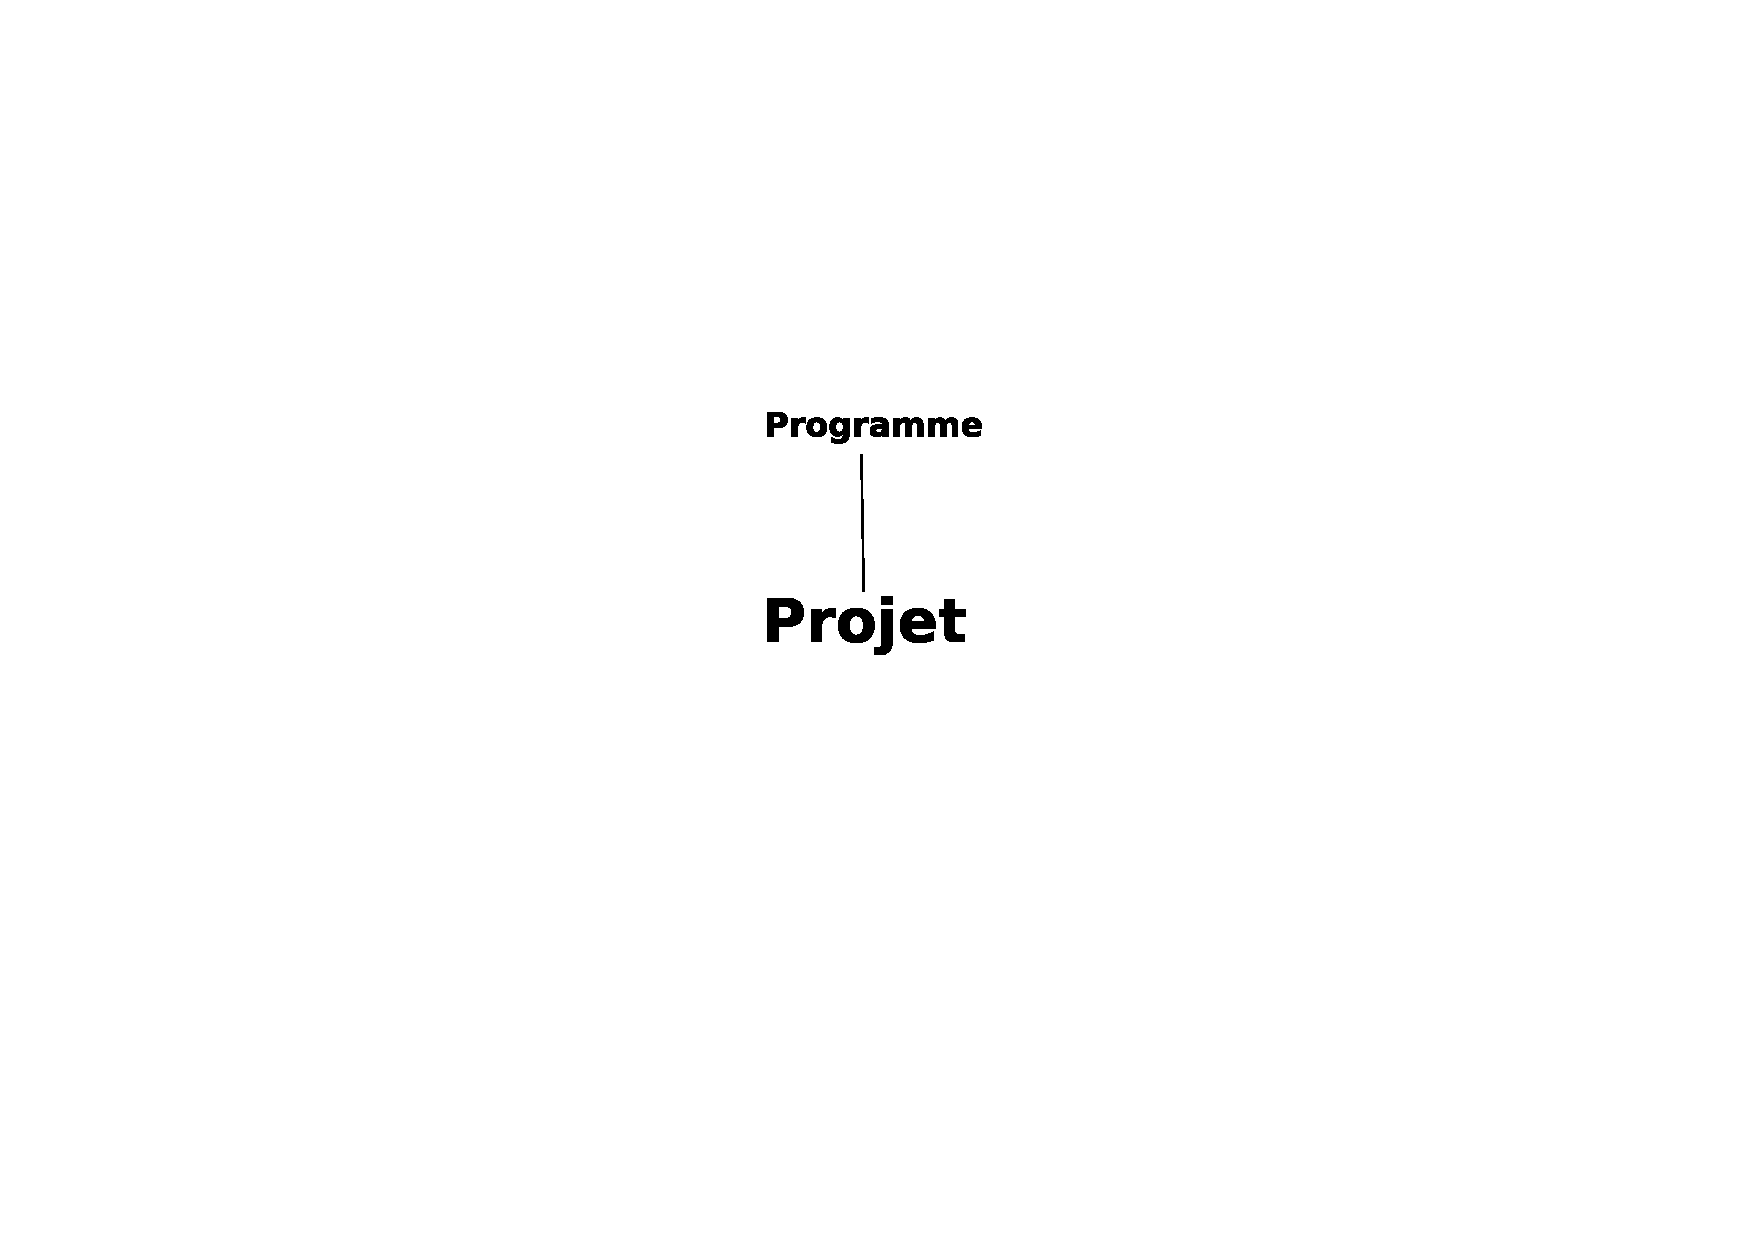
\includegraphics[height=200px]{brainstorming-2.pdf}}
      % Votre projet, c’est de concevoir un programme. Ah, c’est un peu plus
      % précis.
      \only<3>{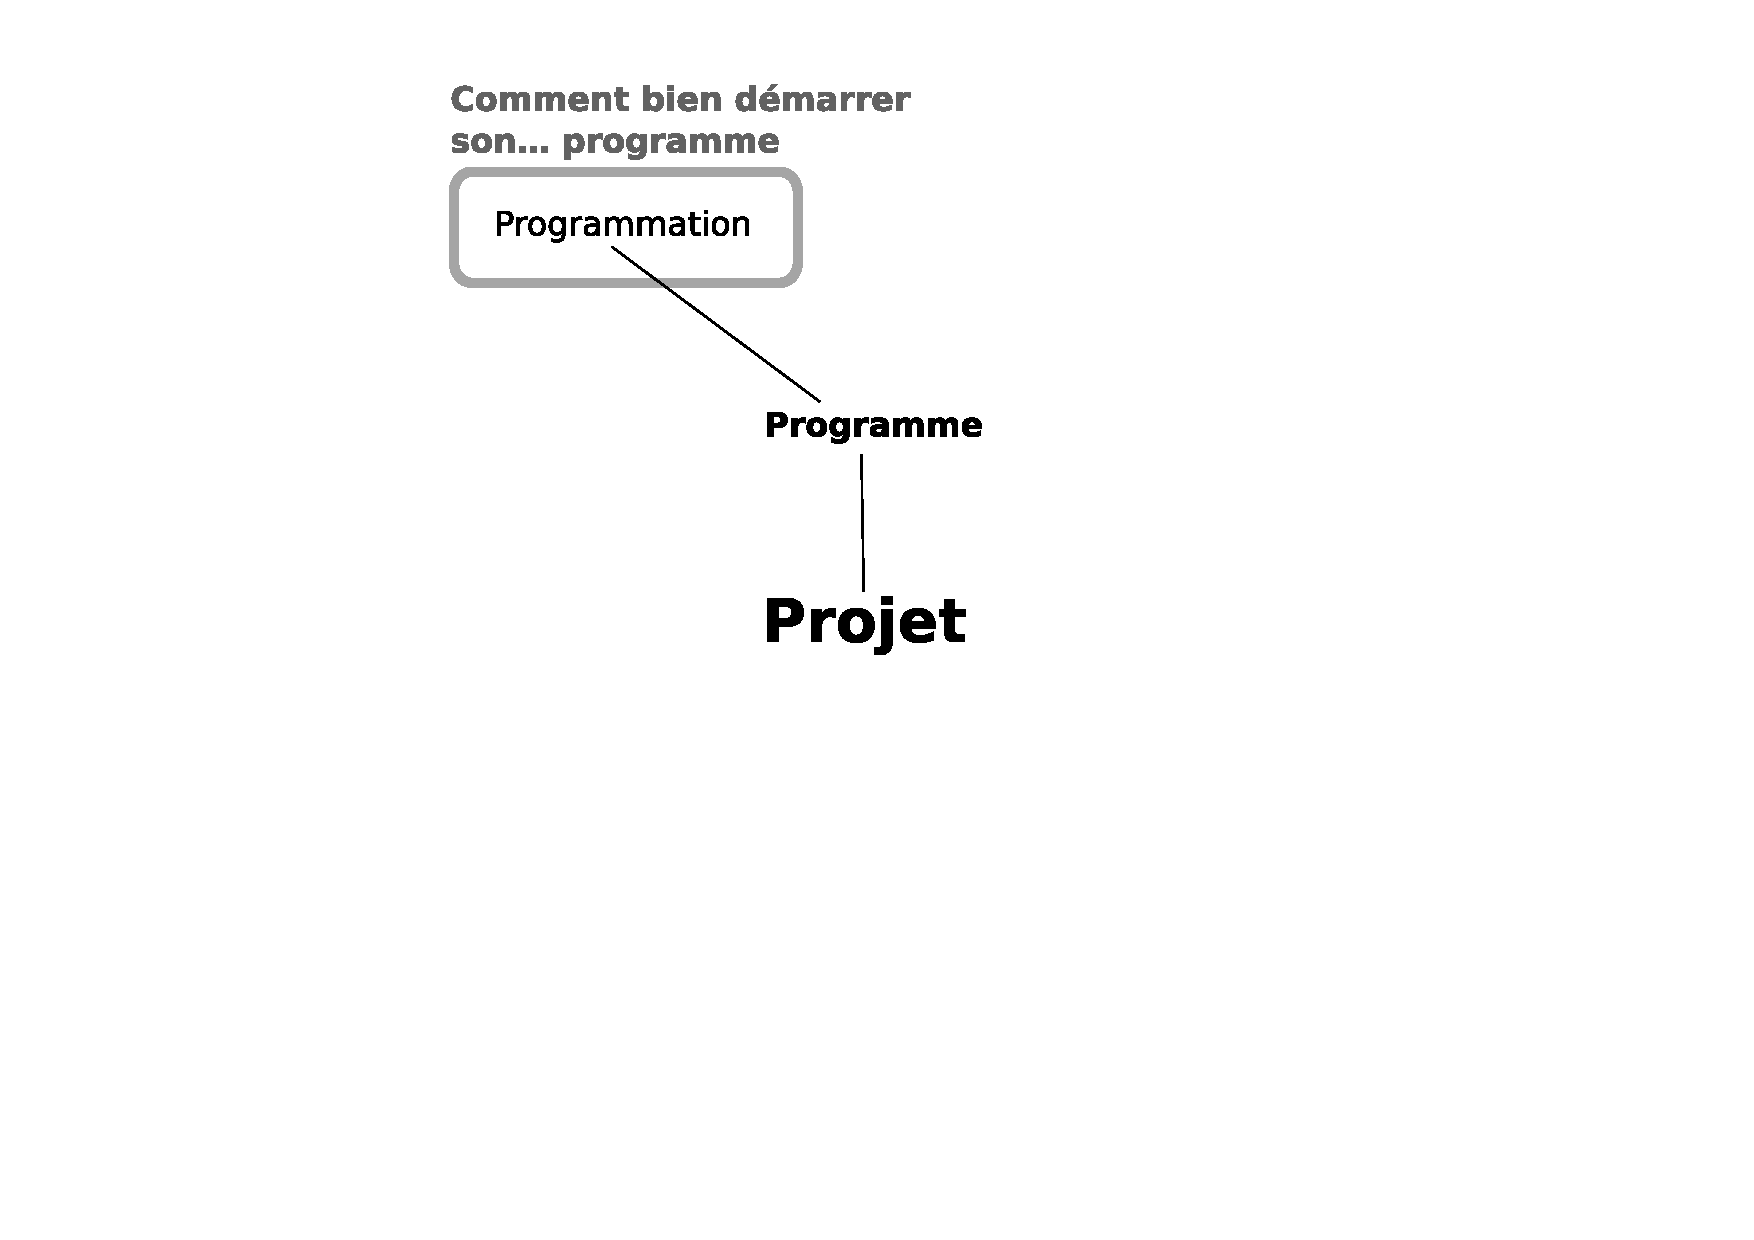
\includegraphics[height=200px]{brainstorming-3.pdf}}
      % Du coup, il va falloir que vous programmiez un peu. Logique. C’est le
      % premier volet de cette conférence : comment allez-vous vous y prendre ?
      \only<4>{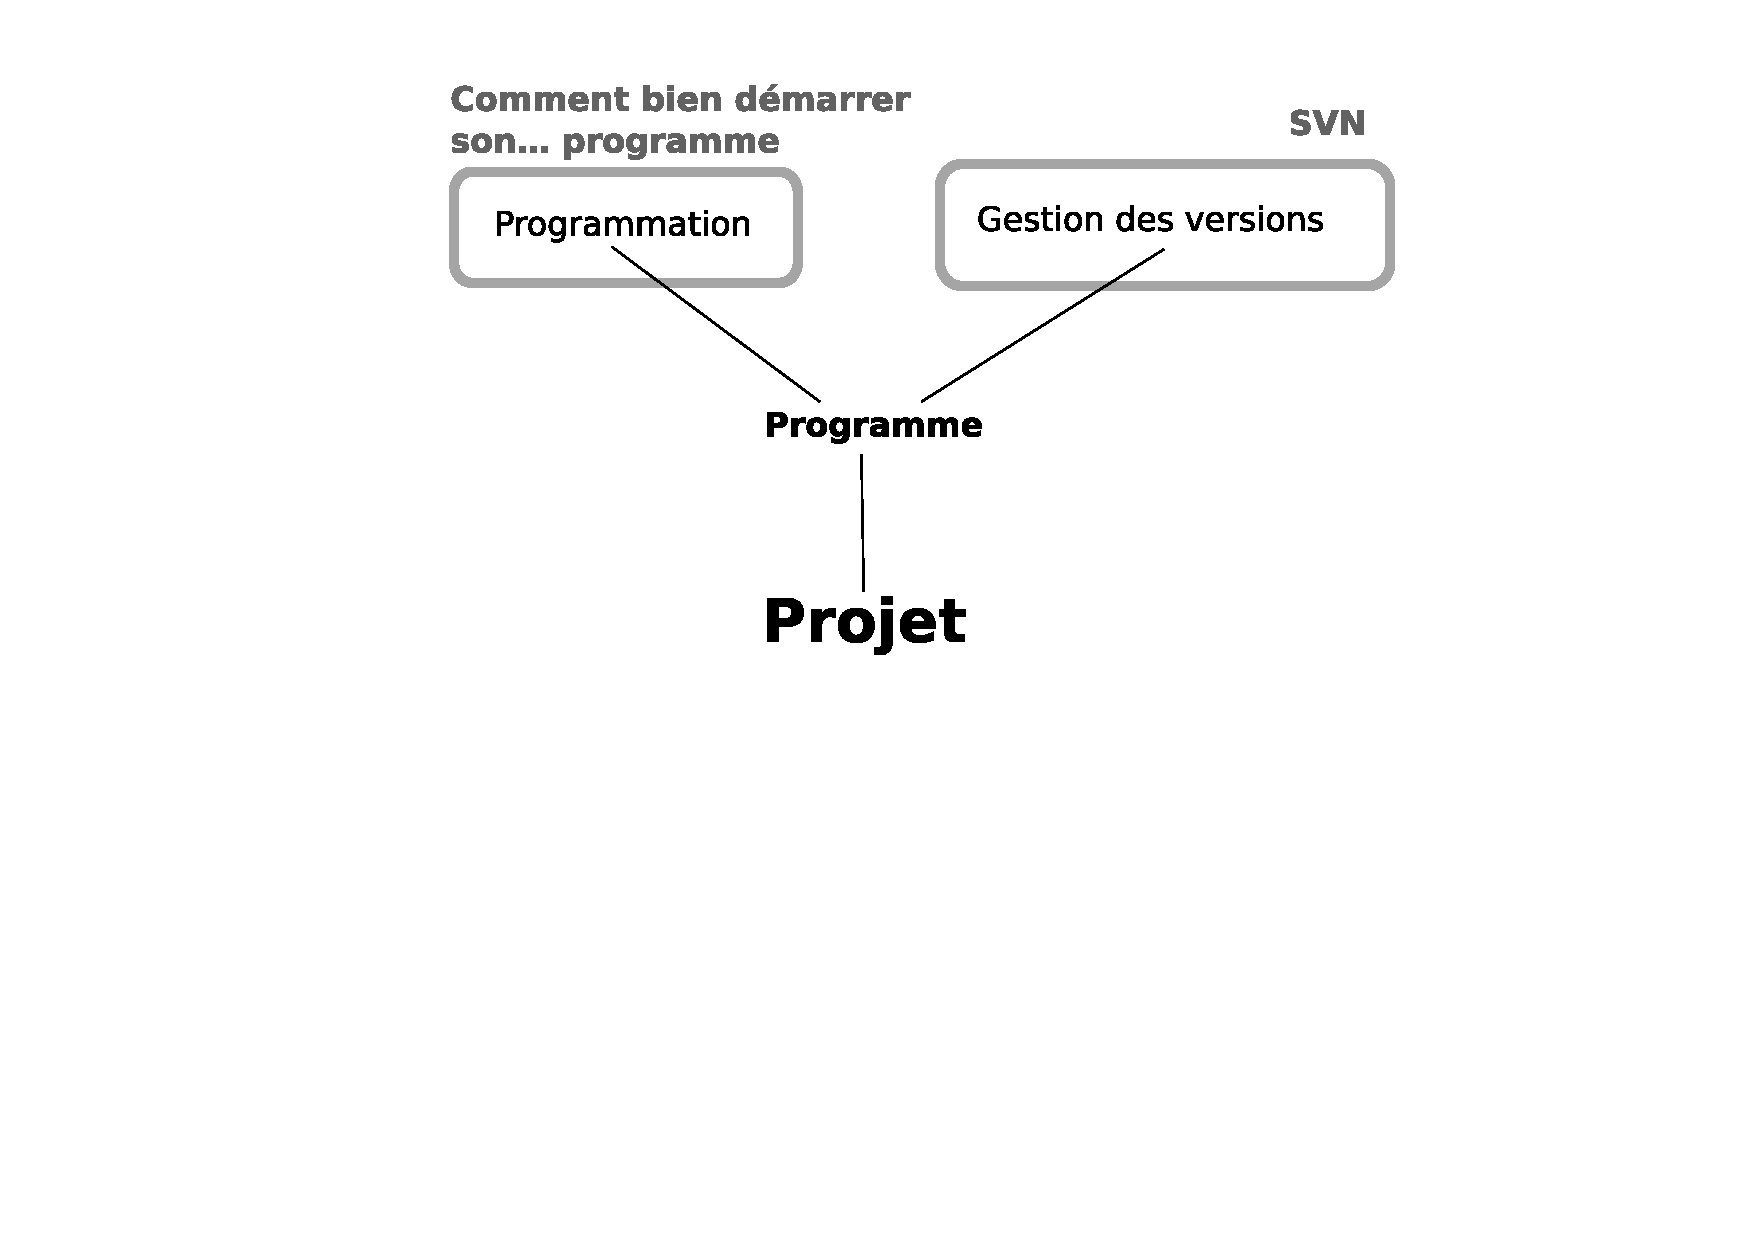
\includegraphics[height=200px]{brainstorming-4.pdf}}
      % Le code, c’est bien, mais… il faut maîtriser son évolution ! SVN, Git,
      % Mercucial et d’autres sont là pour vous faciliter la tâche. La deuxième
      % partie de cette conférence porte sur le principe et l’utilisation de SVN.
      \only<5>{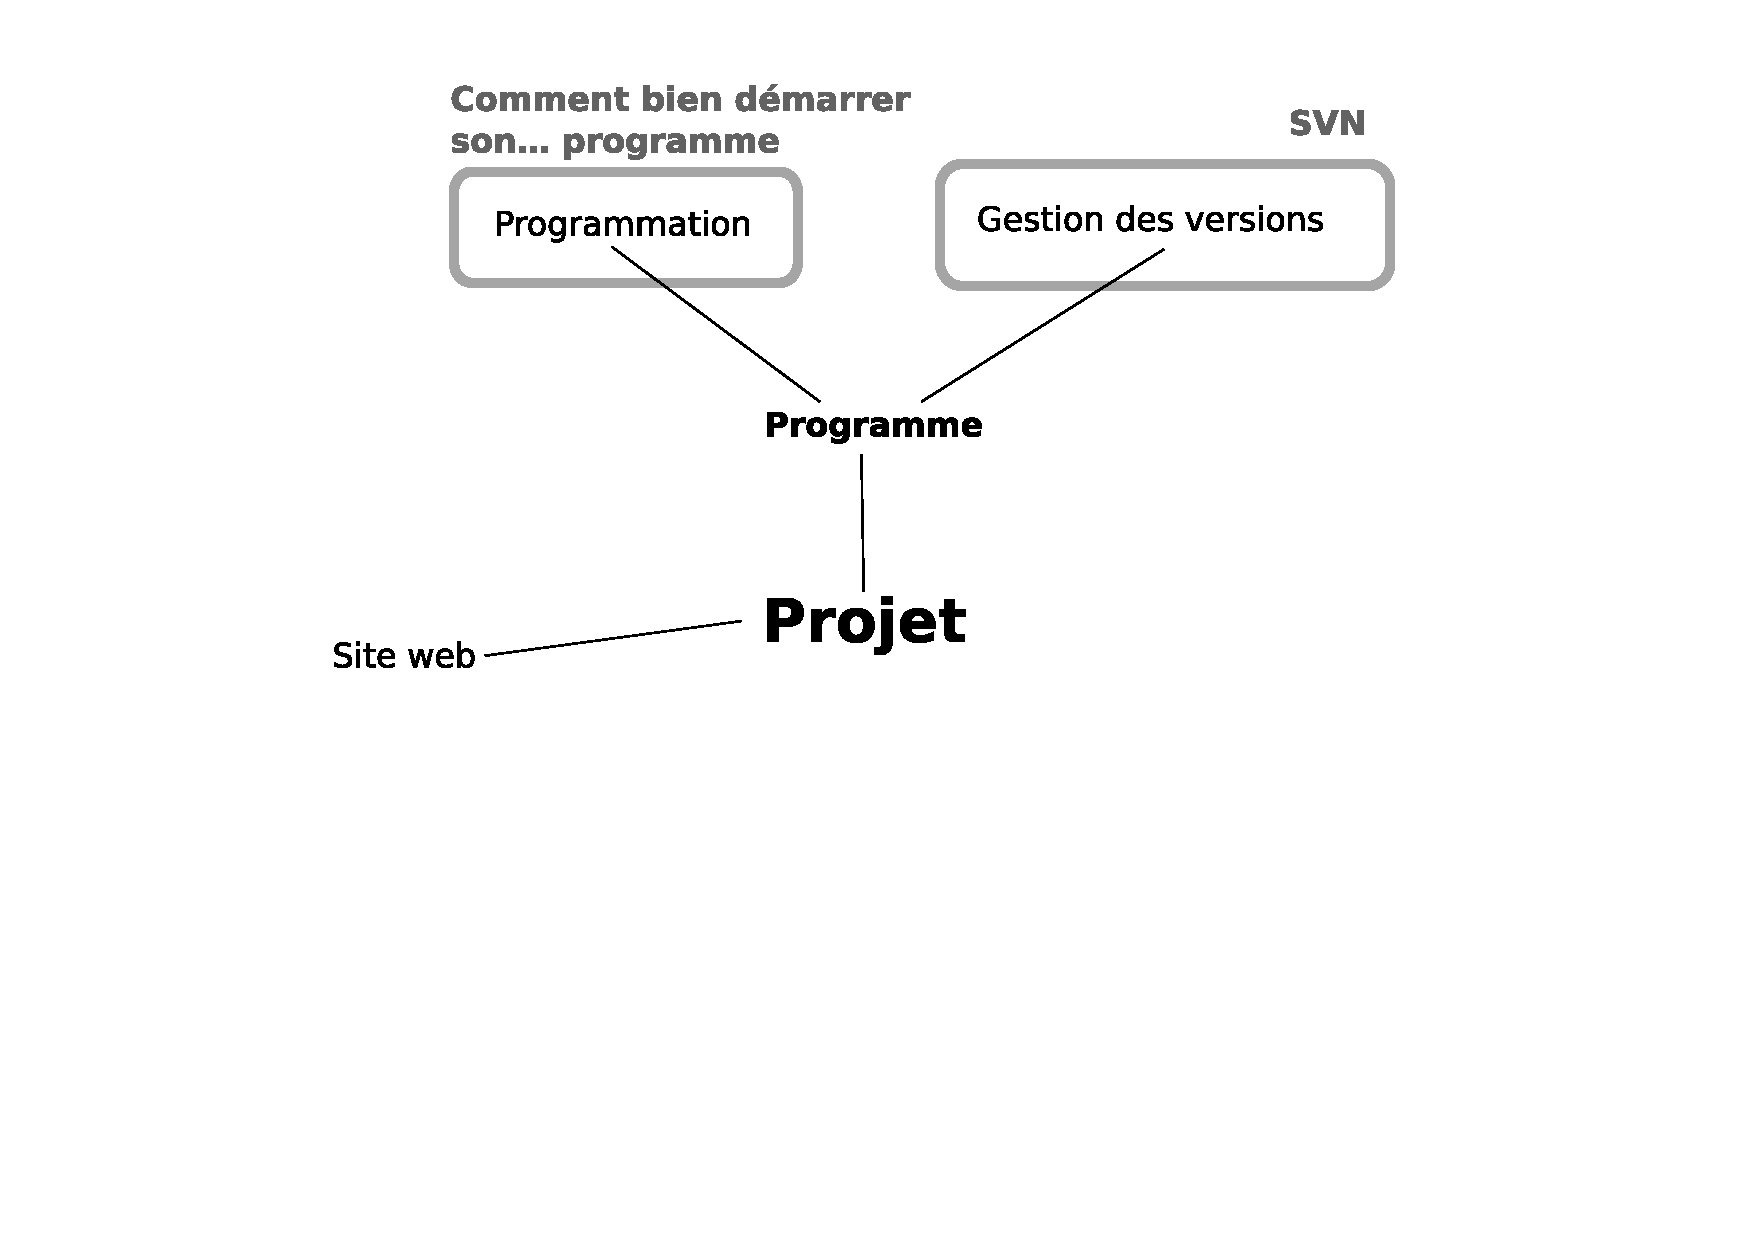
\includegraphics[height=200px]{brainstorming-5.pdf}}
      % Bon, le projet exige que vous concoctiez aussi un site web, une vitrine
      % de votre projet. Le site est assez important, comme toute la
      % communication autour de votre projet, mais ça reste simple et facile à
      % faire… Débrouillez-vous ! :-)
      \only<6>{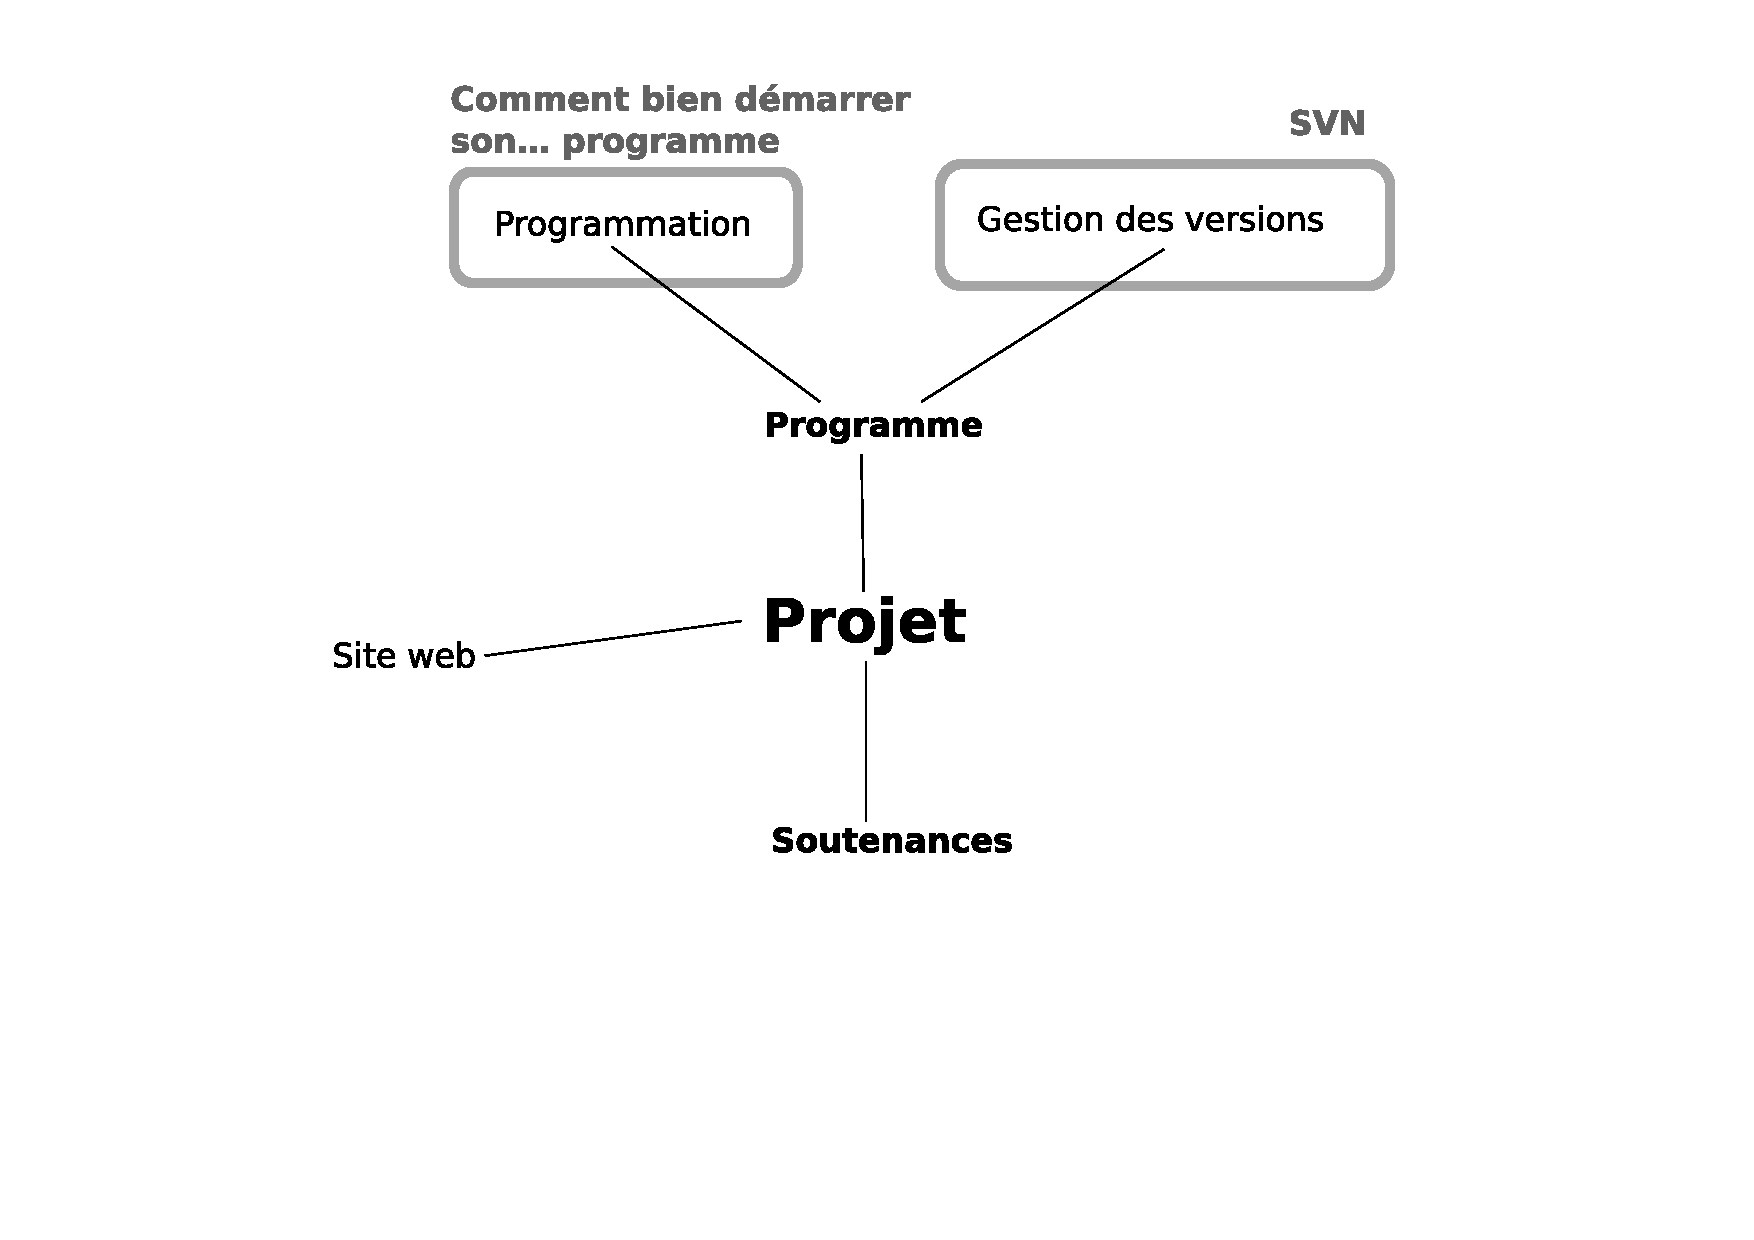
\includegraphics[height=200px]{brainstorming-6.pdf}}
      % Krisboul vous donne du travail et veut vous observer pour être certain
      % que vous bossez ! C’est pour cela que 4 soutenances sont prévues tout au
      % long de l’année.
      \only<7>{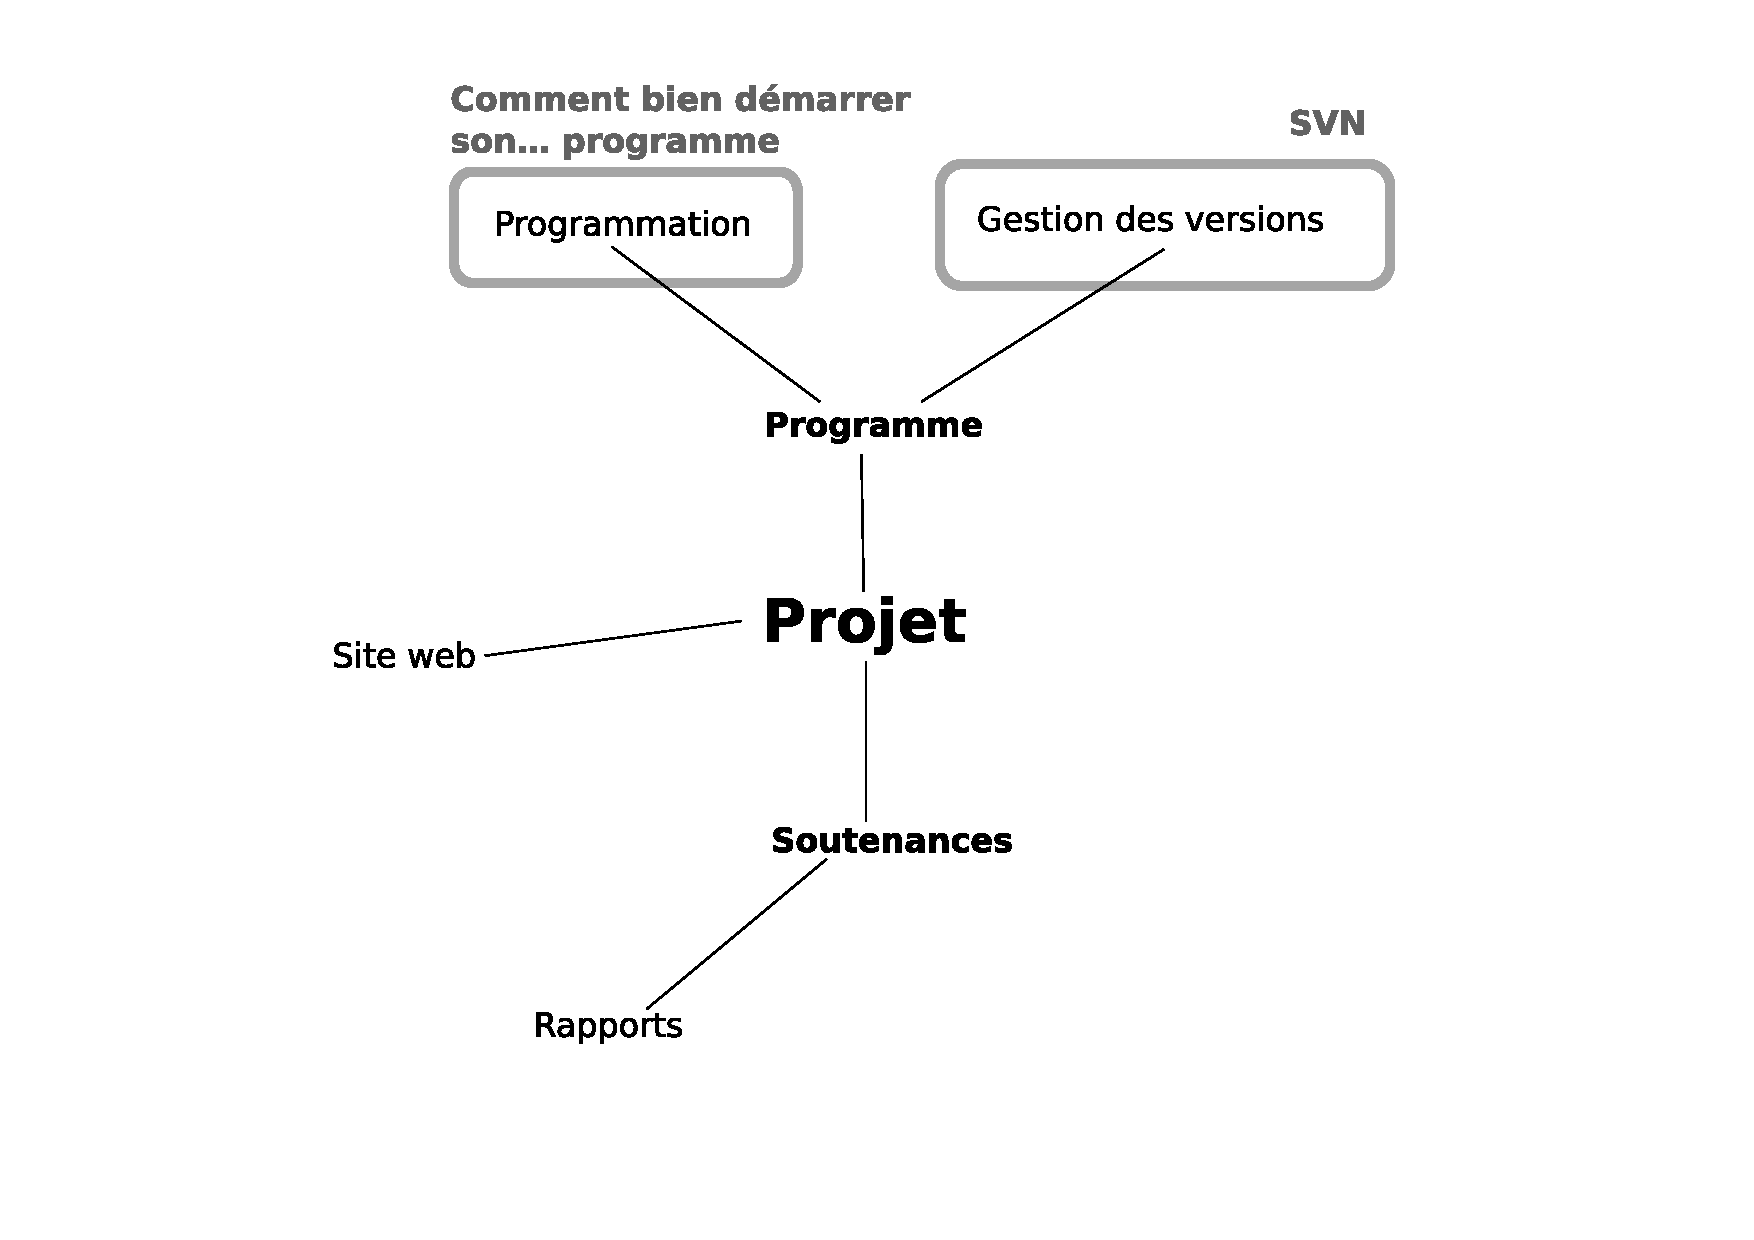
\includegraphics[height=200px]{brainstorming-7.pdf}}
      % À chaque soutenance, vous avez un rapport à fournir…
      \only<8>{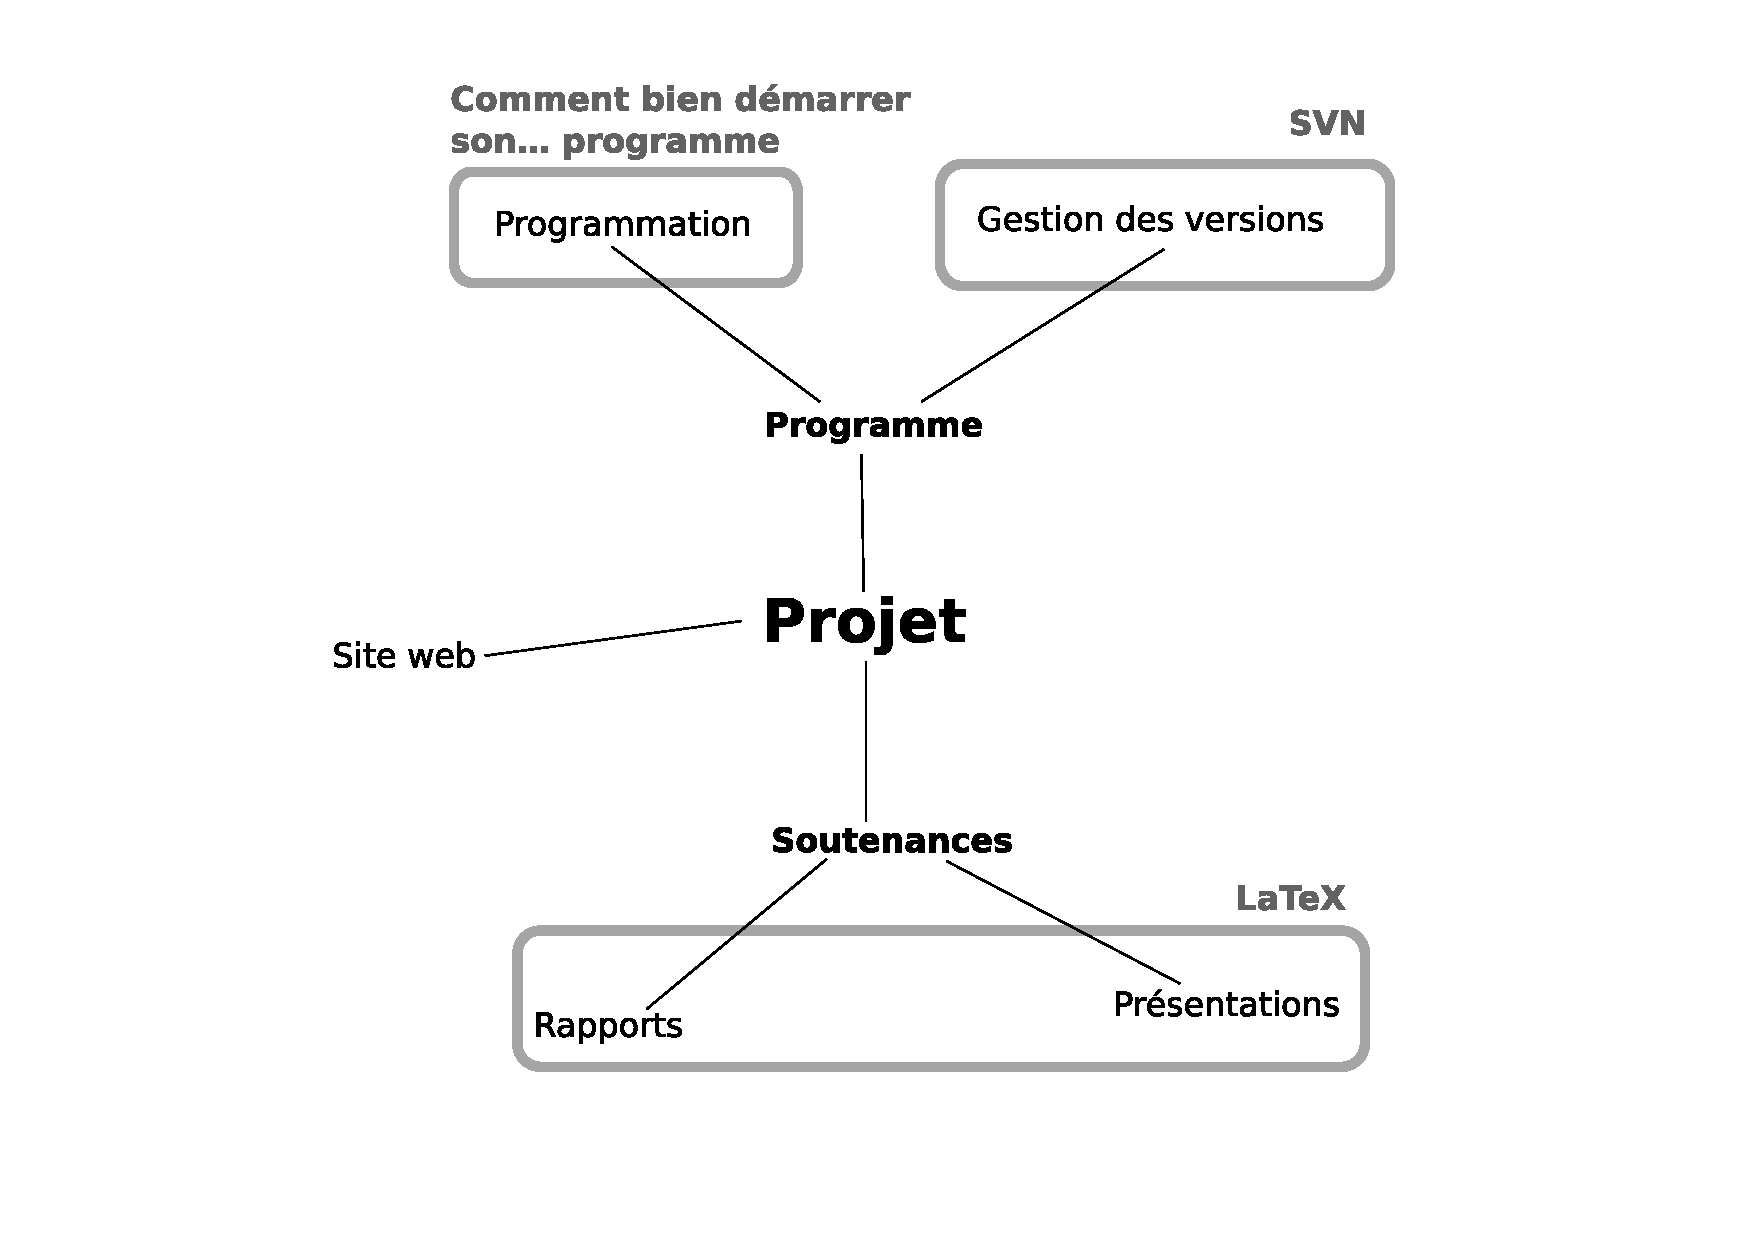
\includegraphics[height=200px]{brainstorming-8.pdf}}
      % … ainsi qu’une présentation à faire. Le contenu n’est pas l’objet de la
      % conférence (c’est dans le sujet, le reste n’est que quelques conseils
      % qu’on peut vous donner), en revanche nous vous conseillons d’utiliser
      % LaTeX pour mettre en forme vos rapports et vos diaporamas.
      \only<9>{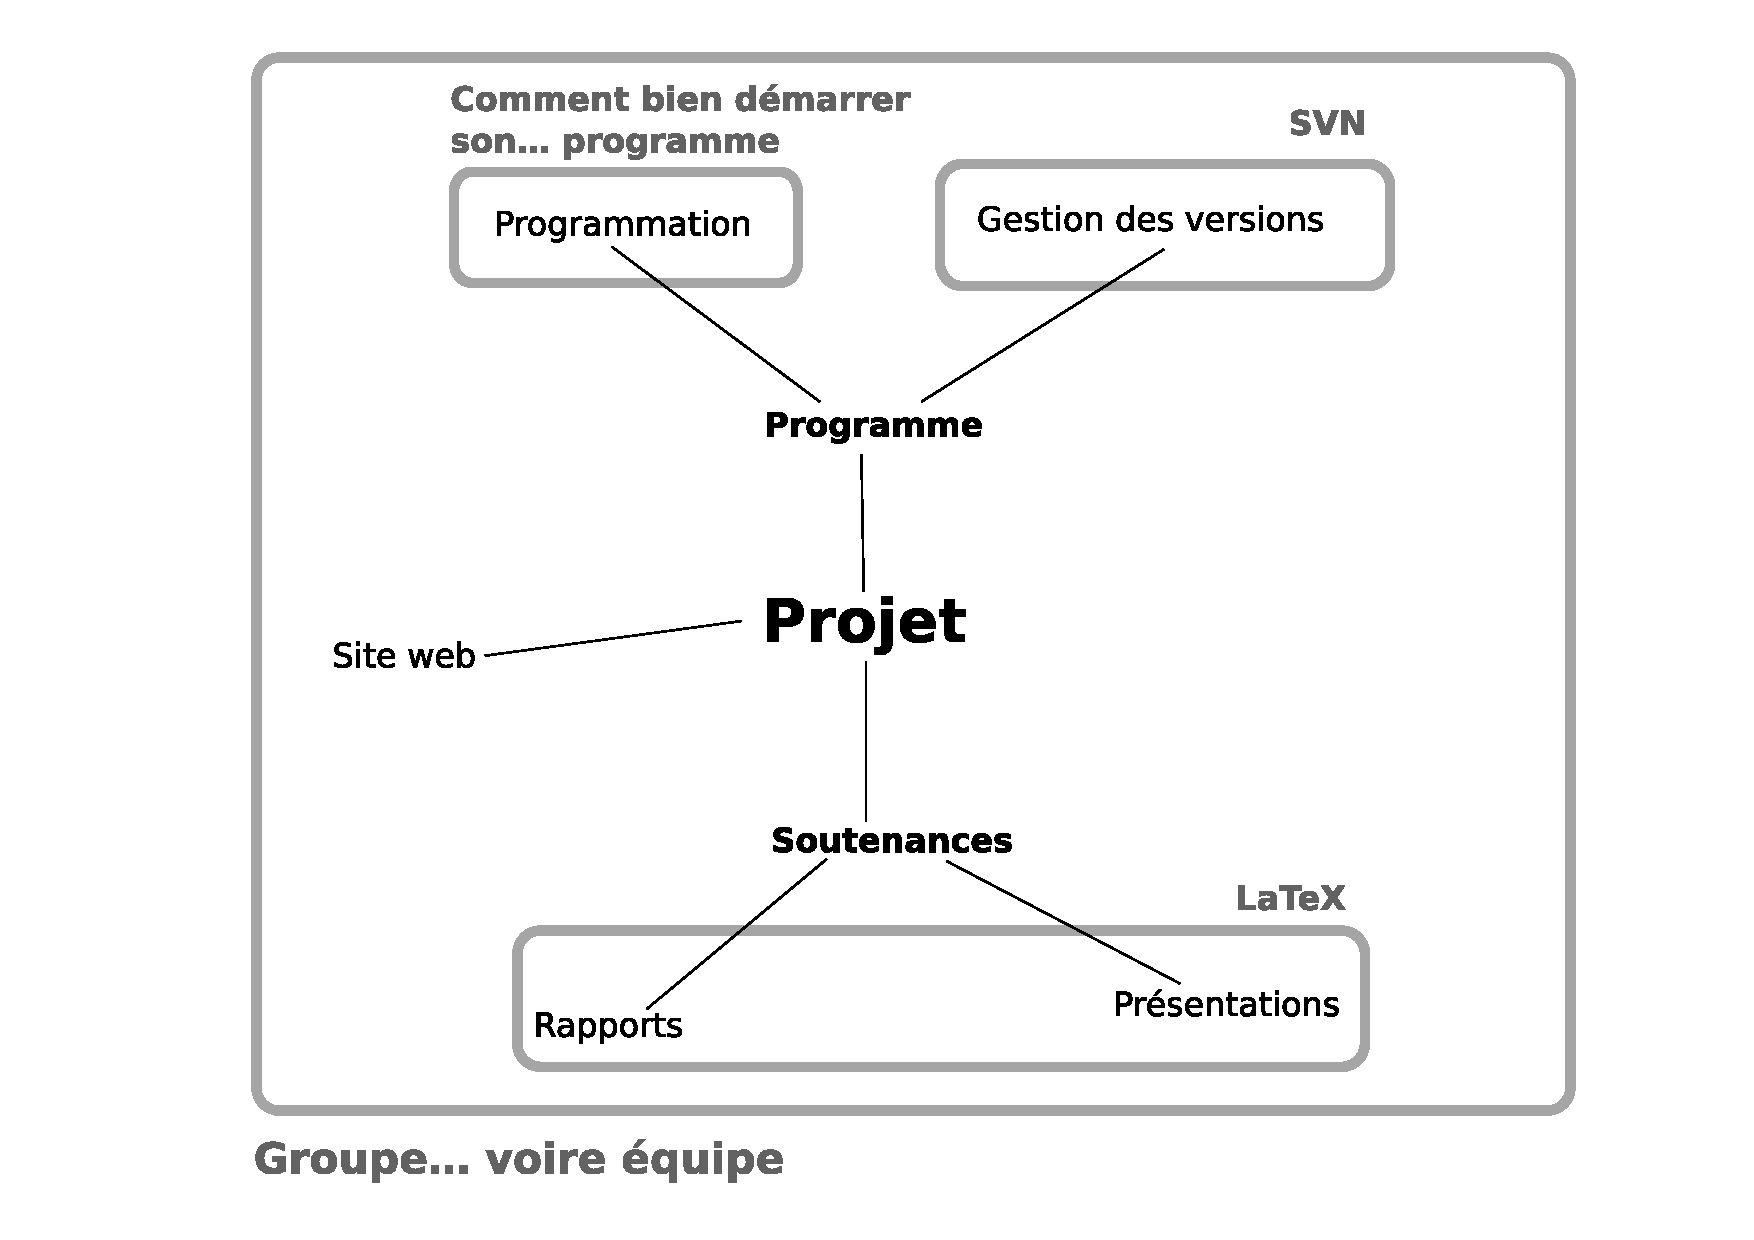
\includegraphics[height=200px]{brainstorming-9.pdf}}
      % Tout ce qui touche à votre projet est à faire en équipe. La gestion de
      % l’équipe est extrêmement importante ! … mais ce n’est pas ici qu’on va
      % vous expliquer comment vous y prendre.

    \end{overlayarea}
  \end{center}
\end{frame}


%\AtBeginSection{
%  \begin{frame}
%    \tableofcontents[currentsection]
%  \end{frame}
%}

%%%
% Conférence « Comment bien démarrer son projet »
% Vendredi 13 novembre 2009
% Partie « Programmation » par Pierre-Marie de Rodat
%%%

\section{Programmation}

\subsection{Deux approches pour découper son projet}
\begin{frame}
  \begin{center}
    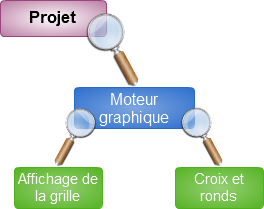
\includegraphics[scale=0.6]{images/slide1.png}
	% Une première approche : découper son projet au feeling en plus petites
	% parties. En prenant l’exemple d’un morpion, on peut distinguer une IA,
	% un moteur de jeu, graphiques, etc. Et ensuite on redécoupe ces moteurs,
	% avec l’exemple du moteur graphique entre affichage de la grille et des
	% pions.
	% Problème : il faut déjà savoir comment marche un projet pour savoir à
	% peu près comment découper et où aller.

	% TODO: refaire le graphique en incluant l’exemple du morpion de manière
	% visuelle.
  \end{center}
\end{frame}

\begin{frame}
  \begin{center}
    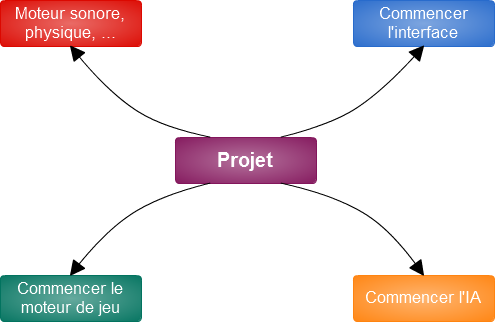
\includegraphics[scale=0.5]{images/slide2.png}
	% Découper le projet entre ce que chacun a envie de faire et chacun le
	% fait dans son coin. Quand on veut tout raccorder, à l’approche de la
	% soutenance, alors c’est l’emmerde. Va falloir réécrirer du code et
	% repenser pour interfacer son code avec celui des autres.
  \end{center}
\end{frame}

\begin{frame}
  \begin{block}{Un mix des deux}
    \begin{itemize}
      \item On découpe un maximum en réfléchissant avant de coder,
      \item chacun prend une partie et sait à peu près où il va,
      \item on reste dynamique.
    \end{itemize}
	% Meilleure méthode : essayer de penser avant de se mettre à coder à
	% l’architecture du projet. Définir les parties importantes, les
	% subdiviser et donner les parties les plus importantes au(x) plus
	% fort(s) ou selon les envies des gens.
	% Faire une base très solide et stable, sinon ça va être bancal, et au fur
	% et à  mesure des soutenances ça va devenir de pire en pire.
	% Essayer de se regrouper par paire : (un bon, un moins bon), le bon peut
	% travailler sur les parties les plus avancées et le moins bon peut
	% toujours demander de l’aide. Les deux connaissent bien leur partie.
  \end{block}
\end{frame}


%%%
% Conférence « Comment bien démarrer son projet »
% Vendredi 03 décembre 2010
%%%

\section{Subversion}

\subsection{Généralités}
\begin{frame}{Pourquoi versionner~?}
  \begin{alertblock}{Concrètement}
    SVN vous permet de~:
    \begin{itemize}
      \item gérer votre code source,
      \item conserver une trace toutes les modifications,

      \item revenir en arrière,
      \item travailler à plusieurs en partageant le code intelligement.
    \end{itemize}
  \end{alertblock}
  \begin{center}
    
\includegraphics[scale=3]{images/logo_svn}
  \end{center}
  % Versionnement : permet de garder un trace de toutes les modifications
  % effectuées sur le code source. Possibilité de revenir en arrière,
  % travailler tous sur les même fichier sans conflit. Ajouter des
  % commentaires aux changements.
  % TODO: virer les référence à SVN là, c’est valables pour tous les VCS,
  % l’introduit juste après, « le plus simple ... » ?
\end{frame}

\subsection{Utilisation typique}

\begin{frame}
  \begin{center}
    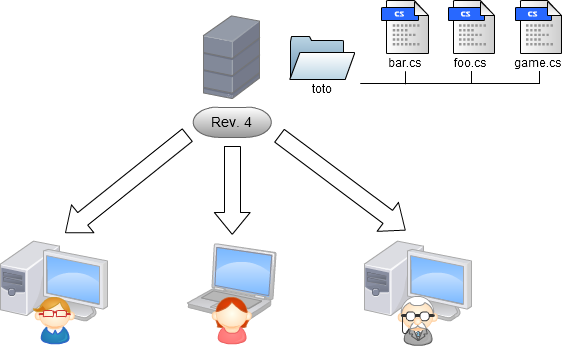
\includegraphics[scale=0.52]{images/1-CheckOut.png}
	% Présentation du dépôt avec les trois fichier versionnés, du numéro de
	% révision. Checkout : récupère tout le contenu du dépot sous la dernière
	% version disponible.
  \end{center}
\end{frame}

\begin{frame}
  \begin{center}
    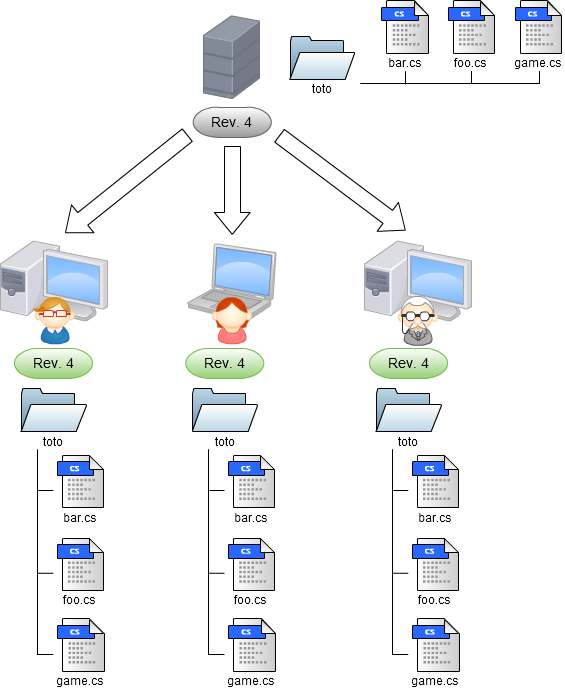
\includegraphics[scale=0.3]{images/2-CheckOut.png}
	% Checkout fini : ils ont tous le contenu du dépôt, ils ont la dernière
	% version, révision 4.
  \end{center}
\end{frame}

\begin{frame}
  \begin{center}
    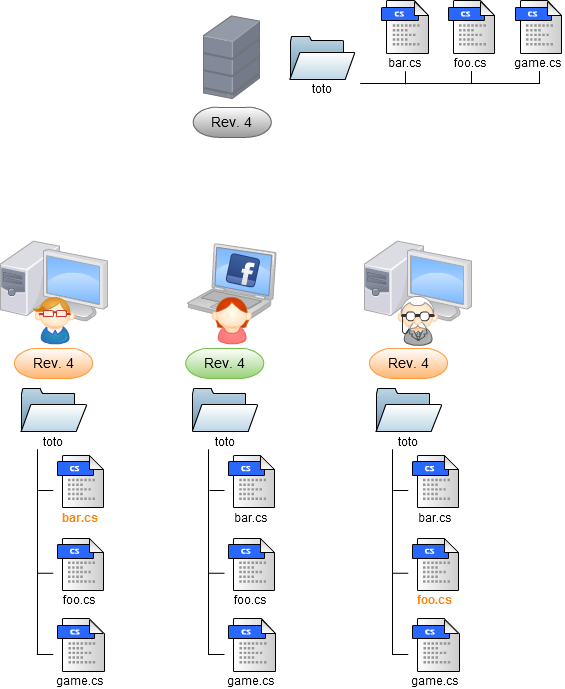
\includegraphics[scale=0.3]{images/3-Work.png}
	% Ils commencent à travailler sur les fichiers qui veulent. Il se sont
	% bien réparti les tâches : la femme et sur Facebook et les deux gars
	% travaillent chacun sur un fichier.
  \end{center}
\end{frame}

\begin{frame}
  \begin{center}
    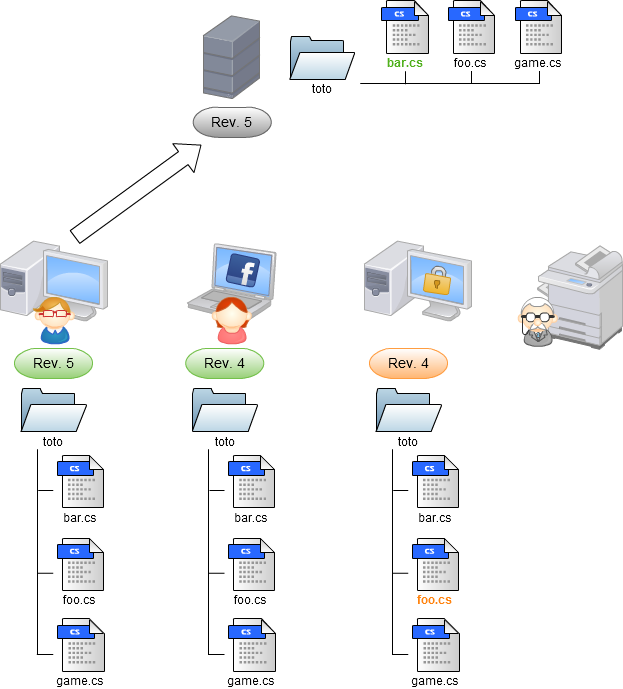
\includegraphics[scale=0.3]{images/4-Commit1.png}
	% Quand le premier a fini son travaille, ça compile, ça marche, il va
	% commit : il va envoyer ses modifications sur le dépôt. Lui et le dépôt
	% passent en révision 5, les autres restent en révision 4. Les autres sont
	% occupés ailleurs.
  \end{center}
\end{frame}

\begin{frame}
  \begin{center}
    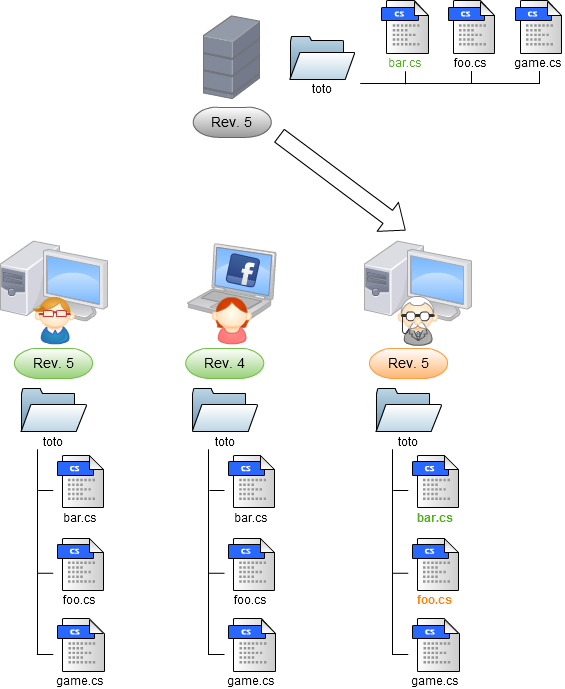
\includegraphics[scale=0.3]{images/5-Update.png}
	% Le vieux revient et veux envoyer son travail. Mais avant de l’envoyer,
	% il fait un update : il récupère les modifications récentes depuis le
	% dépôt. Met à jour juste les fichiers modifiés sur le dépôt, ses
	% modifications locales ne changent pas.
  \end{center}
\end{frame}

\begin{frame}
  \begin{center}
    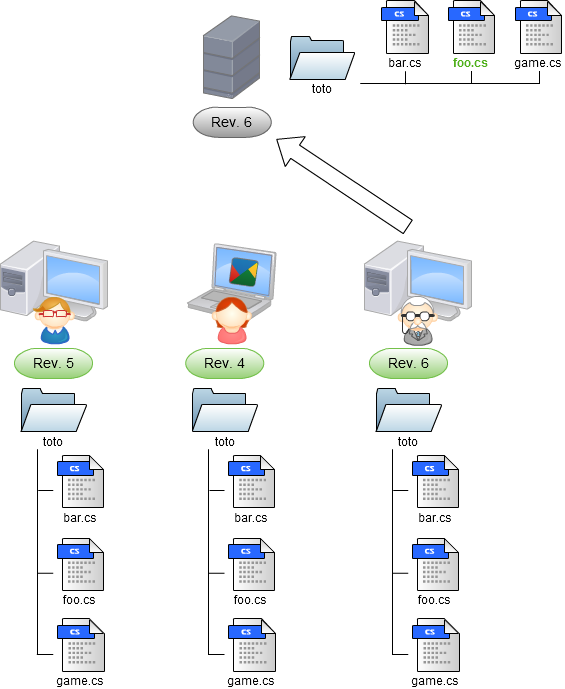
\includegraphics[scale=0.3]{images/6-Commit2.png}
	% Le vieux envoie sont travail, le serveur passe en révision 6, le jeune
	% et la fille ne sont pas au courant.
	% La fille est passé sur Google Buzz.
  \end{center}
\end{frame}

\begin{frame}
  \begin{center}
    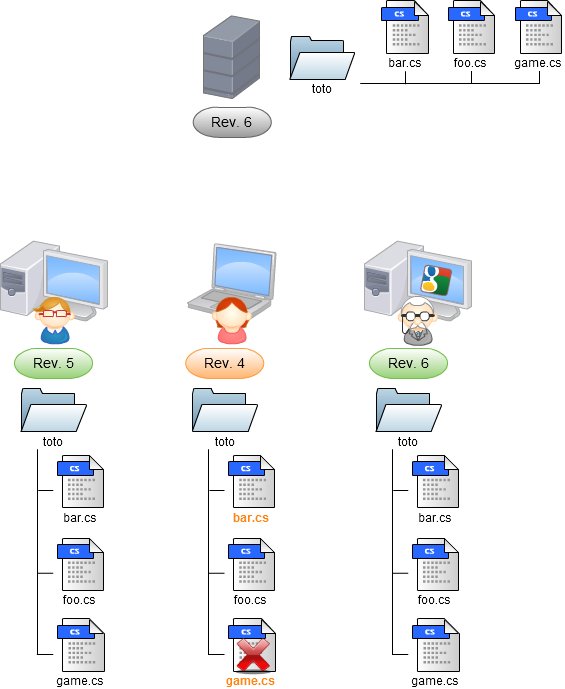
\includegraphics[scale=0.3]{images/7-Work.png}
	% Elle décide de se mettre au travail et décide de supprimer game.cs par
	% ce que ça ne sert à rien selon elle.
	% Le vieux fait des recherches sérieuses sur Google pour le projet.
  \end{center}
\end{frame}

\begin{frame}
  \begin{center}
    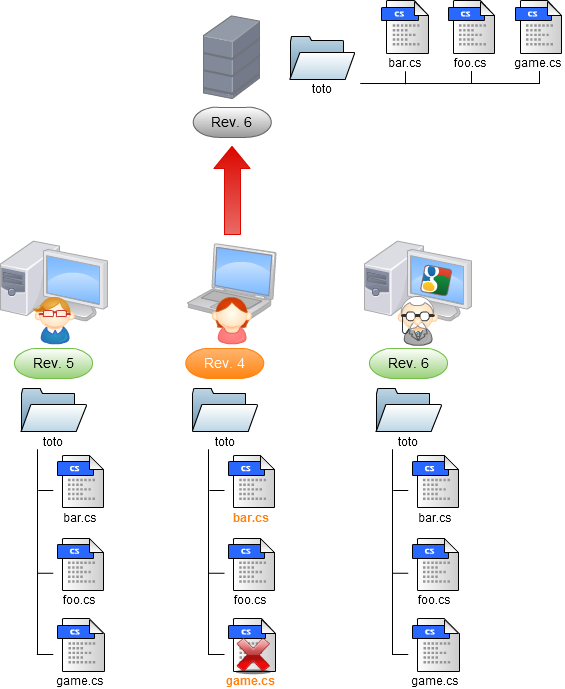
\includegraphics[scale=0.3]{images/8-Commit3.png}
	% La fille essaie de commit comme une bourrine. Erreur ! elle a pas
	% update, le serveur la bloque et lui dit qu’elle n’est pas à jour.
  \end{center}
\end{frame}

\begin{frame}
  \begin{center}
    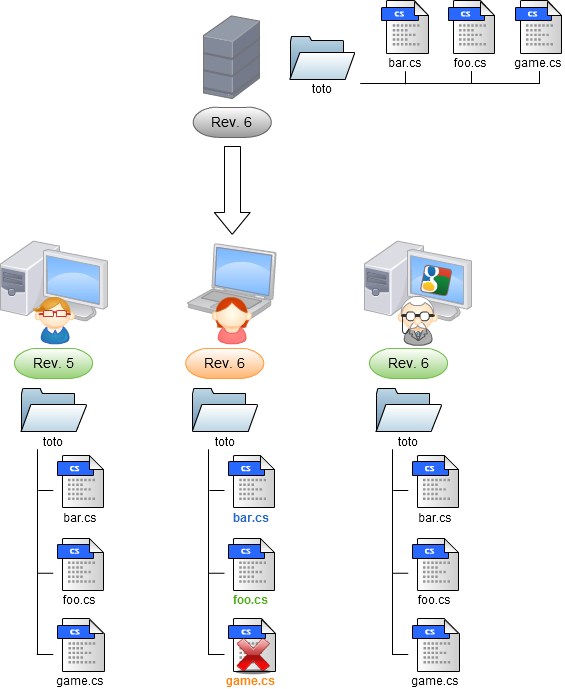
\includegraphics[scale=0.3]{images/9-Update_merge.png}
	% Donc elle commence par update, ça l’amène à la révision 6, tout en
	% gardant ses modifications locales.
	% Et SVN merge bar.cs, ça fusionne les modifications récentes enregistrées
	% par le dépôt ainsi que ses modifications locales et si les deux sont
	% compatibles, il arrive à le faire proprement.
  \end{center}
\end{frame}

\begin{frame}
  \begin{center}
    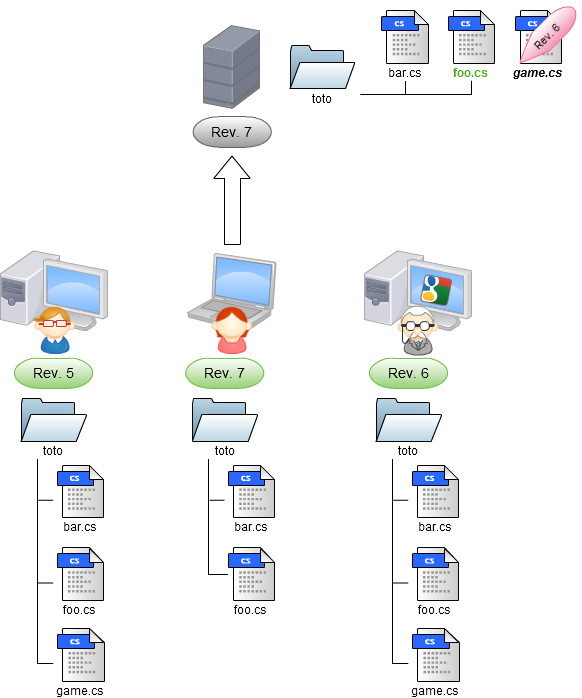
\includegraphics[scale=0.3]{images/10-Commit4.png}
	% Elle commit tout son basard ! game.cs est conservé sur le dépôt par ce
	% qu’il reste une trace de tous les fichiers même supprimé, mais il est
	% n’est pas présent dans la révision actuelle.
  \end{center}
\end{frame}

\begin{frame}
  \begin{center}
    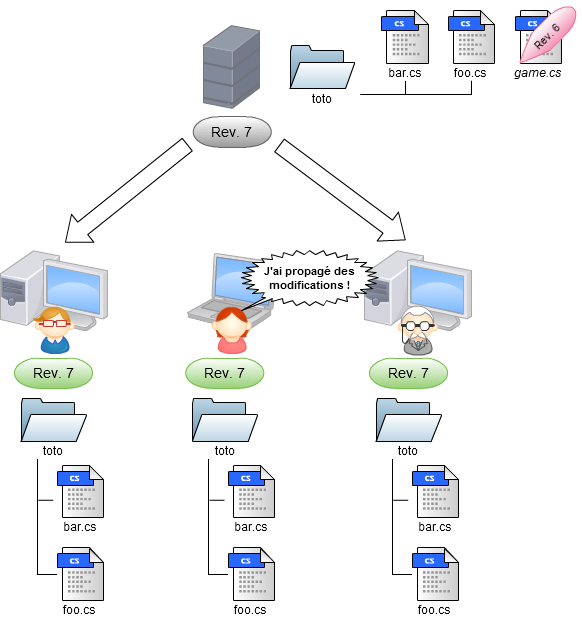
\includegraphics[scale=0.3]{images/11-Update.png}
	% Elle est toute contente (imiter la fille « wahoo j’ai bien travaillé ! »),
	% et dis aux autres d’update. Ils le font et n’ont plus de game.cs
  \end{center}
\end{frame}

\begin{frame}
  \begin{center}
    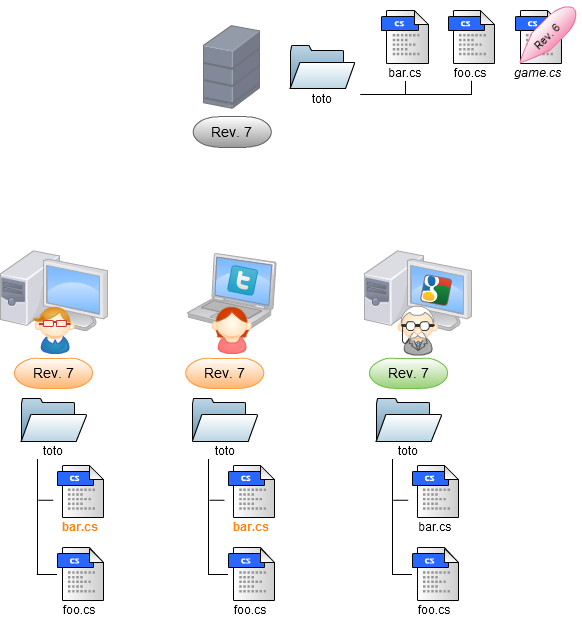
\includegraphics[scale=0.3]{images/12-Work.png}
	% De retour au travail : elle change un truc dans bar.cs et va sur tweeter.
	% Mais ce qu’elle a commit ne compilait pas. Il faut toujours commit un
	% truc qui marche !
	% Le jeune résout le souçit.
  \end{center}
\end{frame}

\begin{frame}
  \begin{center}
    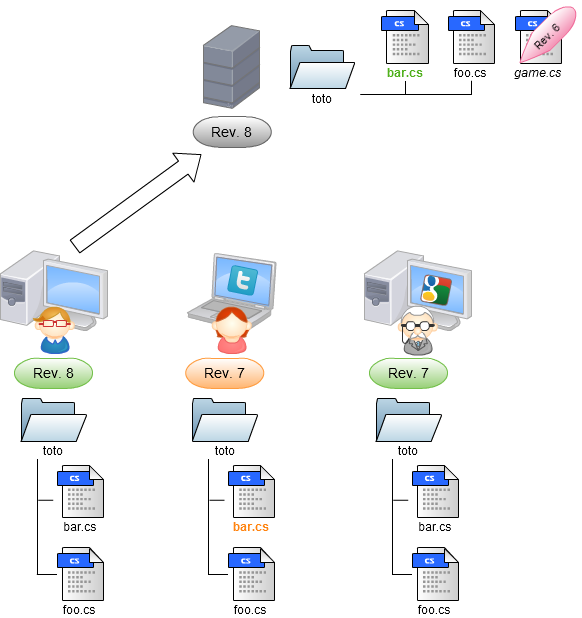
\includegraphics[scale=0.3]{images/13-Commit4.png}
	% Il commit son fix des conneries de la fille.
  \end{center}
\end{frame}

\begin{frame}
  \begin{center}
    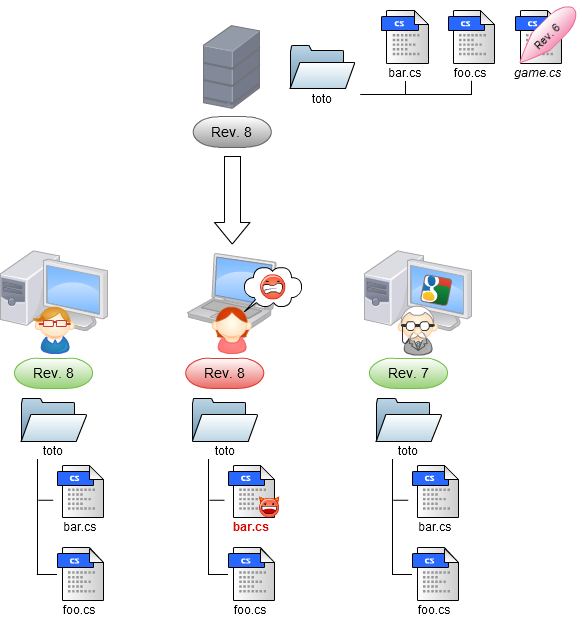
\includegraphics[scale=0.3]{images/14-Conflict.png}
	% La fille veut commiter les changements qu’elle avait fait avant sa
	% session tweeter sur bar.cs, mais a retenu la leçon et update avant. Mais
	% là il y a conflit sur bar.cs, c’est à dire que SVN n’a pas réussie à
	% fusionner leur deux travail, probablement par ce que le jeune et la
	% fille vienne de modifier les même lignes de code.
  \end{center}
\end{frame}

\begin{frame}
  \begin{center}
    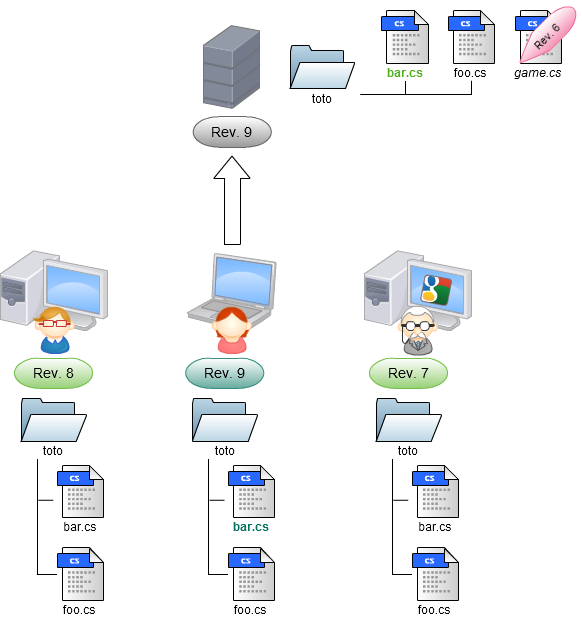
\includegraphics[scale=0.3]{images/15-Resolved.png}
	% Elle résout le contenu d’une façon ou d’une autre : mon truc c’est de la
	% merde, je vais prendre la version qui est sur le dépôt, mon truc c’est
	% le meilleur, les autres c’est des gros cons ou alors essayer de comparer
	% les deux versions et de fusionner à la main (très peu probable pour
	% elle).
	% Elle indique le conflit comme «resolved» et envoie le résultat.
  \end{center}
\end{frame}

\begin{frame}
  \begin{center}
    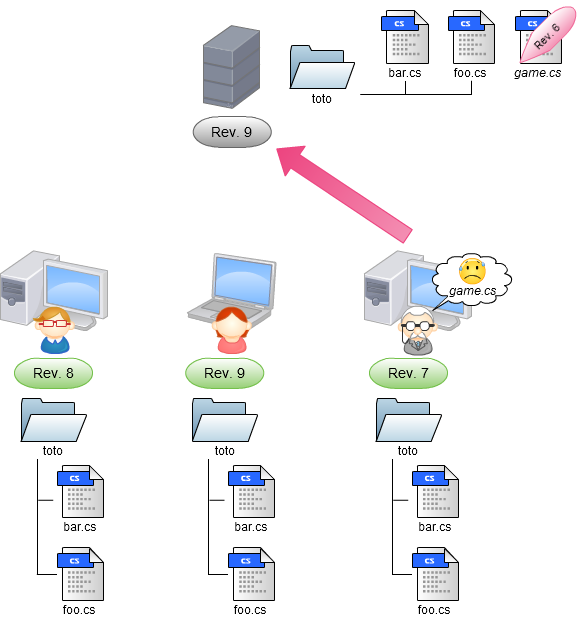
\includegraphics[scale=0.3]{images/16-Back1.png}
	% Le vieux a fini sa recherche et veut travailler sur game.cs mais il se
	% rend compte qu’il a été supprimé. Mais SVN c’est trop bien, il va
	% pouvoir aller récupérer le fichier !
  \end{center}
\end{frame}

% TODO : peut être ajouter un exemple de revert ?
% TODO: ajouter le nom des principales commandes en gros en haut à chaque fois
% qu’elles sont illustrées dans les exemples.

\subsection{Commandes usuelles}

\begin{frame}{Subversion survival package}
  \begin{block}{Checkout -- co}
    Récupération du contenu d'un dépôt (désigné par une URL) à une version donnée.
  \end{block}
  \begin{block}{Update -- up}
    Mise à jour du contenu d'un dossier/fichier sous versionnement par rapport à la référence.
  \end{block}
  \begin{block}{Commit -- ci}
    Enregistrement des modifications effectuées sur le serveur.
  \end{block}
  \begin{block}{Add / delete}
    Activer et désactiver le versionnement sur un dossier/fichier.
  \end{block}
  % Les quatres commandes pour survivre. On peut tout faire avec.
  % Checkout : bien pour récupérer le dépôt au départ mais aussi quand vous en
  % avez marre, que plus rien de marche, vous supprimez tout et vous re-checkout
  % le dépôt en entier.
  % Update : récupère les mise à jour.
  % Commit : envoyer ses modifications.
  % Add / delete : ajouter et supprimer des fichiers au dépôt. Il faut commit
  % après et vos fichiers seront ajouter au versionnement.
\end{frame}



\subsection{Environnement de travail}
\begin{frame}
  \begin{center}
    
\includegraphics[scale=0.35]{images/logo_tortoise}
  \end{center}
  \begin{alertblock}{TortoiseSVN}
    \begin{itemize}
    \item S'intégre parfaitement à Windows,
    \item Ajout d'action sur les fichiers et dossiers (clic droit),
      \item Modification visuelle pour les dossiers et fichiers sous versionnement.
      \end{itemize}
	  % Permet d’avoir une interface complètement intégrée et simple
	  % d’utilisation, avec de gros boutons.
    \end{alertblock}
\end{frame}

\begin{frame}
  \begin{figure}
    \begin{center}
      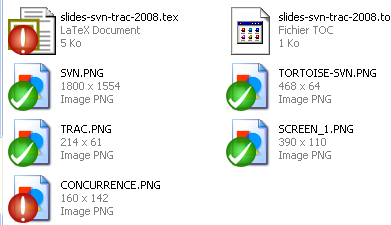
\includegraphics[scale=0.7]{images/dirView}
	  % Rouge : fichier modifié localement, les modif n’ont pas été envoyées
	  % sur le dépôt. Vert : fichier à jour avec le dépôt. Rien : pas
	  % versionné, le fichier et ses modifications ne sont pas envoyées sur le
	  % serveur.
    \end{center}
  \end{figure}
\end{frame}
\begin{frame}
  \begin{figure}
    \begin{center}
      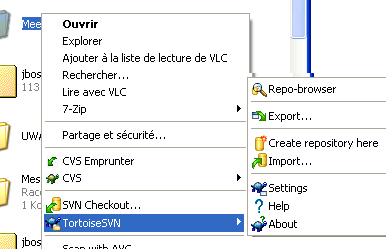
\includegraphics[scale=0.7]{images/actions}
	  % Menu intégré à l’explorateur, avec toutes les fonctions qu’on a
	  % décrite accessibles facilement.
    \end{center}
  \end{figure}
\end{frame}

\subsection{Bonnes pratiques}
\begin{frame}
  \begin{alertblock}{Update}
    Effectuer des updates régulièrement.
  \end{alertblock}
  % Update très régulièrement
  \begin{alertblock}{Commit}
    Commiter \textbf{régulièrement} du code qui \textbf{compile}.
  \end{alertblock}
  % On update toujours avant de commit et quand on commit on fait toujours
  % attention que notre merde fonctionne, sinon vous allez être détesté par
  % votre groupe.
  \begin{alertblock}{Add}
    Ne pas mettre sous versionnement~:
    \begin{itemize}
    \item Les fichiers compilés par votre code (.exe, .o, .out, \ldots),
    \item Les fichiers propres à votre environnement de travail,
    \item Les fichiers systèmes (Thumbs.db, \ldots),
    \item Des fichiers inutiles (SVN n'est pas un système de partage de fichiers).
    \end{itemize}
	% On ajoute pas des fichiers compilé, on ajoute pas une vidéo d’intro de
	% 300Mo sinon à chaque fois que quelqu’un va vouloir checkout, il va se
	% tapper la vidéo à télécharger et c’est pas cool.
  \end{alertblock}
\end{frame}

\subsection{Où trouver un dépôt~?}
\begin{frame}
  \begin{exampleblock}{Les dépôts gratuits}
    \begin{itemize}
    \item GoogleCode
    \item SourceForge
    \item Assembla
    \item svn.pc-show.com
    \end{itemize}
	% Vous pouvez trouver des dépôt gratuit chez ces fournisseurs. Ils
	% fournissent tous de bonnes interfaces. Googlecode et Sourceforge sont
	% les mieux. Fournis un wiki qui permet de libérer ses pulsions
	% créatrices, le système de ticket, vous créer un ticket pour chaque bug
	% ou feature manquante et vous pouvez changer son statut et la personne
	% qui doit s’en charger avec des commentaires, ou encore voir le code en
	% ligne.
  \end{exampleblock}
\end{frame}


%%%
% Conférence « Comment bien démarrer son projet »
% Vendredi 03 décembre 2010
%%%

\section{Soutenances}

\subsection{Généralités}
\begin{frame}
  \begin{block}{Points clés}
    \begin{itemize}
    \item Capter l'attention de \emph{Krisboul},
    \item 13 à 15 minutes,
    \item être fier de son jeu,
    \item être en avance sur le planing.
    \end{itemize}
  \end{block}
\end{frame}

\begin{frame}
  \begin{block}{Le site internet}
    \begin{itemize}
    \item La vitrine du projet,
    \item noté dès la deuxième soutenance,
    \item être simple, beau, avec du contenu \textbf{à jour}.
    \end{itemize}
  \end{block}
\end{frame}

\begin{frame}
  \begin{block}{Les rapports}
    \begin{itemize}
    \item \LaTeX,
    \item environ 20 pages,
    \item images, captures, dessins, à donf,
    \item s'inspirer des promos précédentes.
    \end{itemize}
  \end{block}
\end{frame}

\begin{frame}
  Au boulot~!
\end{frame}

\end{document}